\chapter{Sensoren}
\renewcommand{\kapitelautor}{Autor: Lucas Ullrich}

%%%%%%%%%%%%%%%%%%%%%%%%%%%%%%%%%%%%%%%%%%%%%%%%%%%%%%%%%%%%%%%%%%%%%%%%%%%%%%%
\section{Pixy CMUcam5}
Bei der PIXY CMUcam5 handelt es sich um ein Open Source Kameramodul, welches über eine Objekterkennung verfügt. Mit diesem ist es möglich sogenannte Colorcodes oder einfache Objekte zu erkennen.

\begin{figure}[H]
  \begin{centering}
    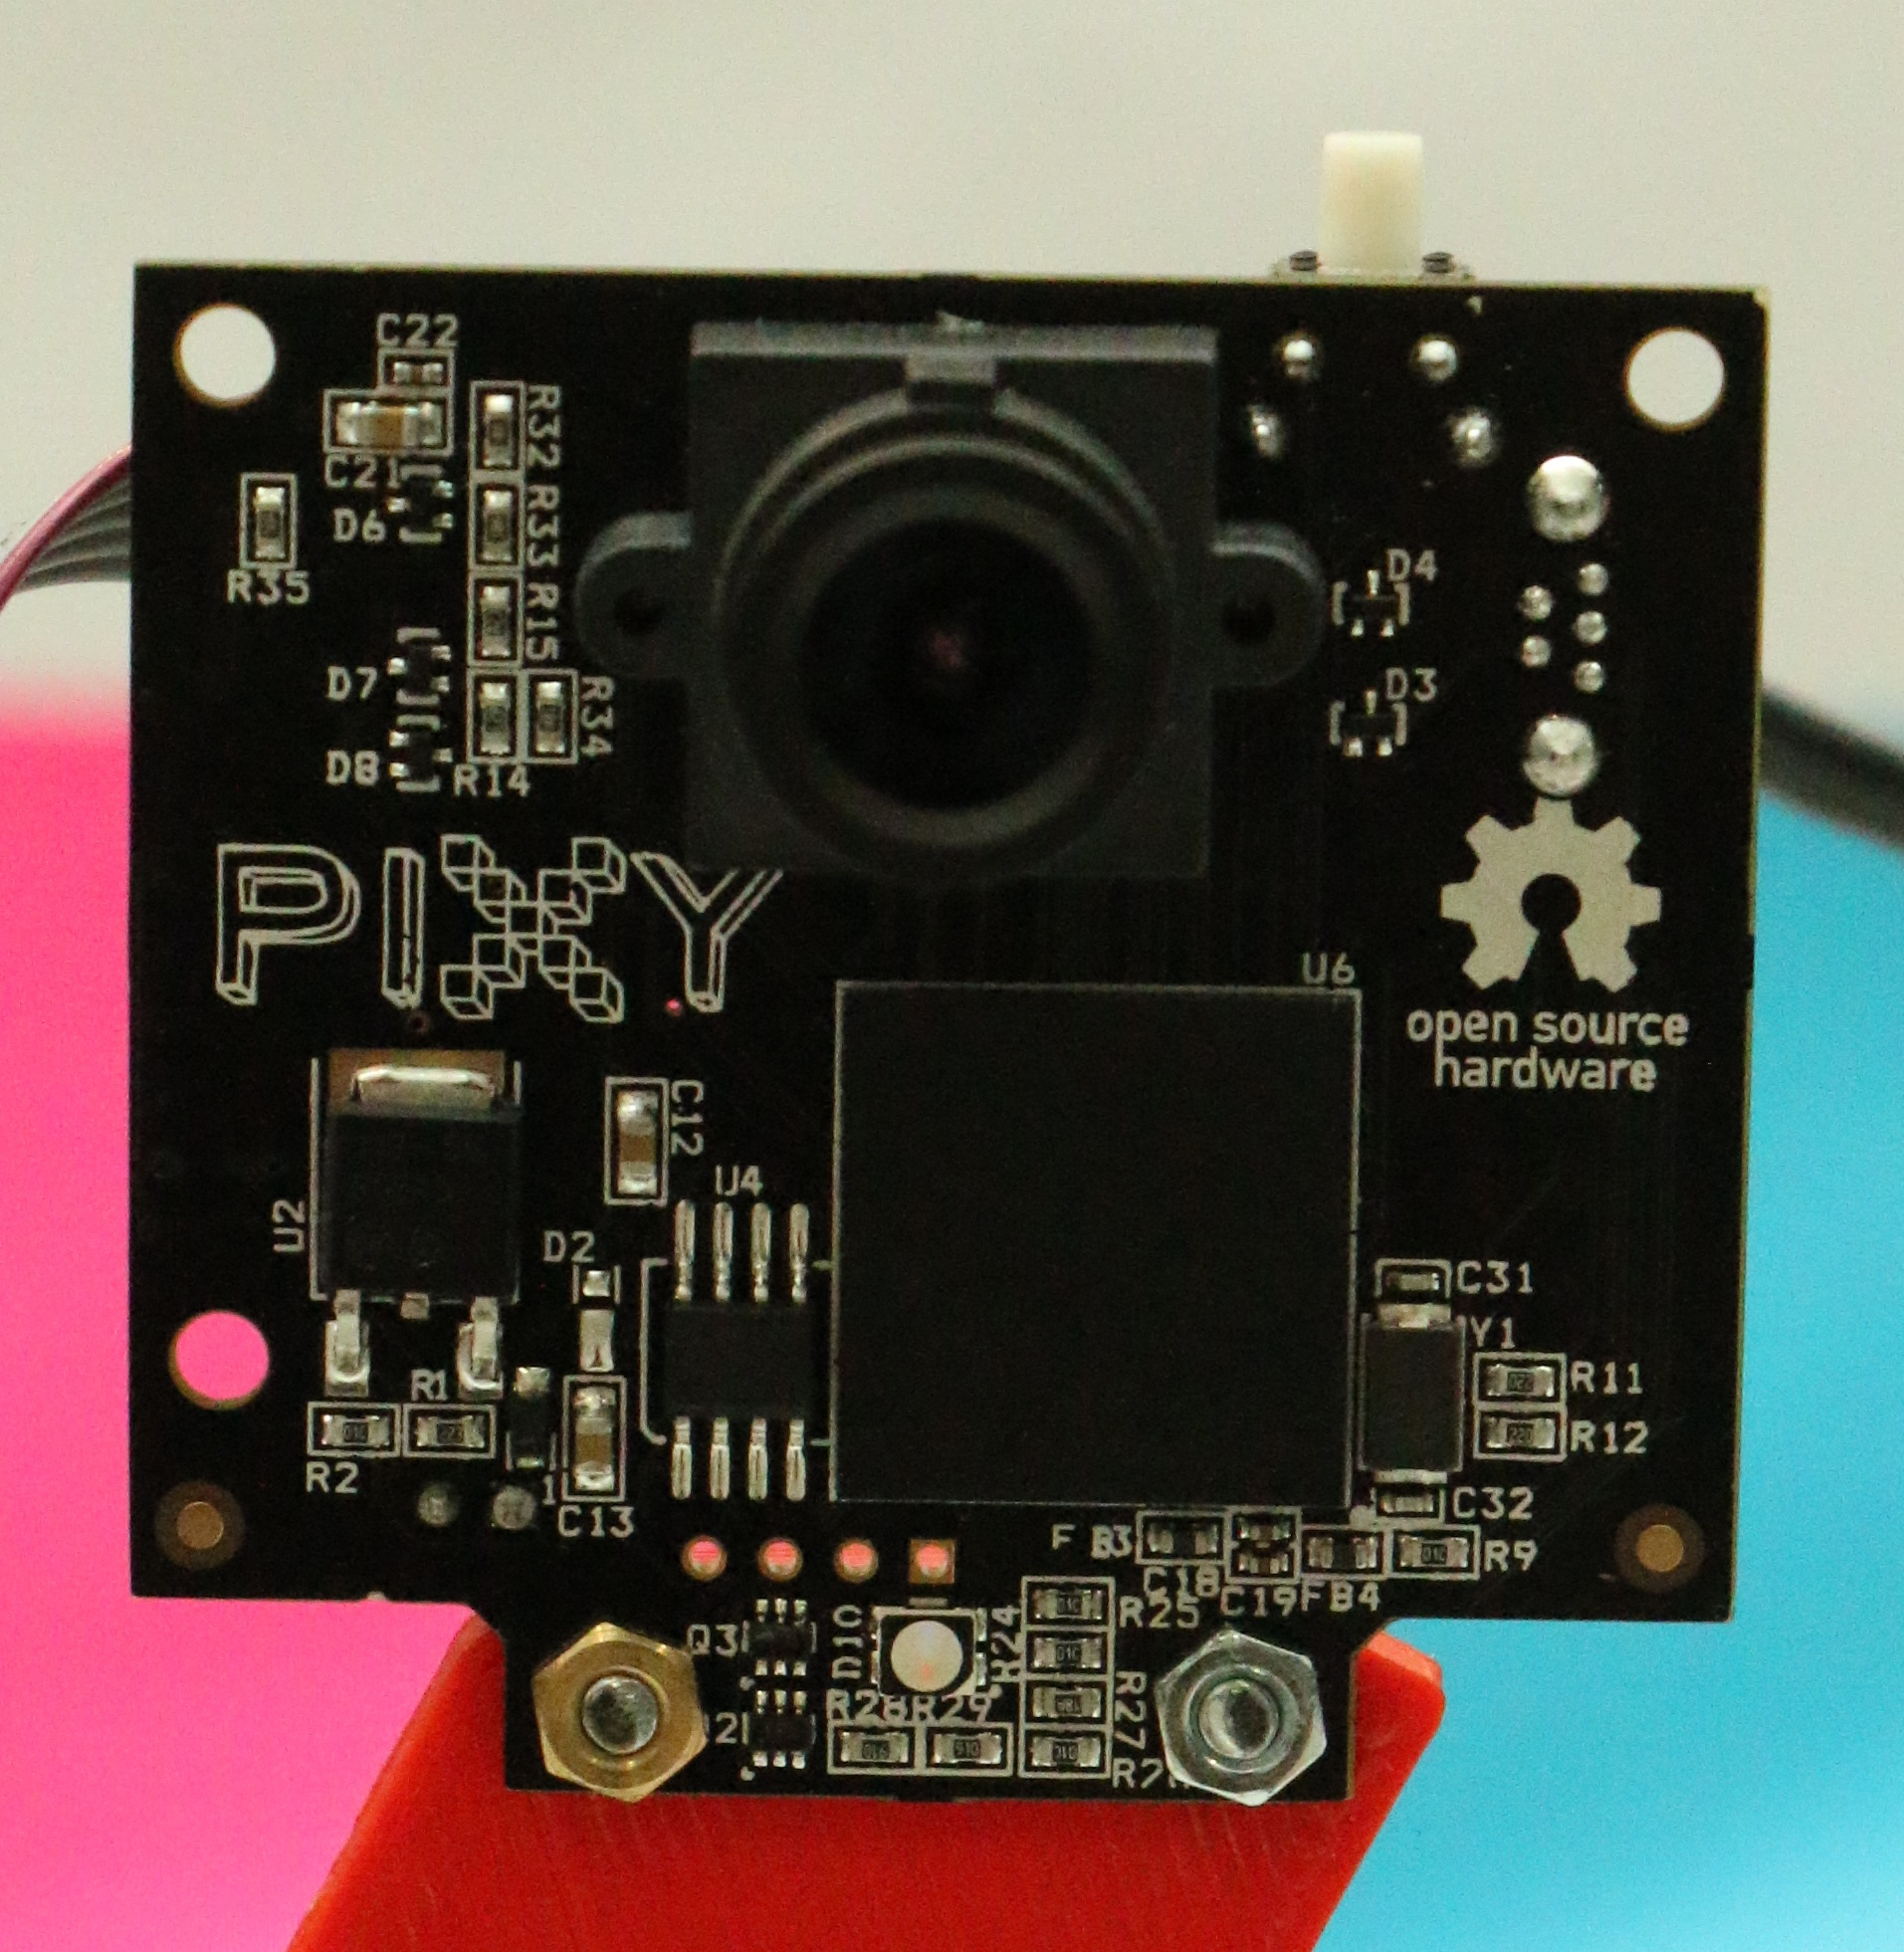
\includegraphics[width = 0.4\textwidth]{Bilder/Pixy_CMUcam5}
  \par\end{centering}
  \caption{PIXY CMUcam5}
  \label{PIXY}
\end{figure}

\begin{figure}[H]
  \begin{centering}
    \subfigure[Colorcode]{
\includegraphics[width = 0.4\textwidth]{Bilder/Colorcode}}
    \subfigure[Objekt]{
\includegraphics[width = 0.4\textwidth]{Bilder/Colorcode}} %%%%%%%%%Objekt statt Colorcode
  \par\end{centering}
  \caption{Erkennbare Objekttypen}
  \label{PIXY_Objekte}
\end{figure}

  \subsection{Technische Planung}
    \subsubsection{Mögliche Verfahren zur Positionserkennung}
    Hier muss grundsätzlich zwischen zwei Messmethoden unterschieden werden:
    \begin{itemize}
      \item \textbf{Absolute Positionsmessung}\\
      Hier wird die Postion von einem gleichbleibenden Punkt aus gemessen. Dabei ist ein konstanter Referenzpunkt wichtig. Verändert sich dieser oder kann die Distanz nicht genau gemessen werden ist die Messung unbrauchbar.

      Für eine absolute Positionsmessung bieten sich diverse Triangulationsverfahren an, diese sind ausgesprochen rechenaufwändig und benötigen meist eine sehr genaue Laufzeitmessung. Für die Triangulation können die unterschiedlichsten Signale verwendet werden, am gängigsten sind jedoch jene die mit elektromagnetischen Wellen arbeiten, \zB WLAN, Bluetooth. Dies bedeutet, dass sich die Signale mit Lichtgeschwindigkeit ausbreiten.

      Bei einer Messung derart schneller Signale muss ein hoher Aufwand betrieben werden um eine Messgenauigkeit von einigen cm zu erzielen. Eine weitere Herausforderung sind Mauern \bzw Hindernisse. Hier muss ständig berücksichtigt werden wo ein Objekt steht und ob der geplante Weg überhaupt frei ist.
      \item \textbf{Relative Positionsmessung}\\
      Hier wird die Position von einem wechselnden Punkt aus gemessen. Um hier eine Positionierung im Raum ermöglichen zu können, ist es erforderlich immer zu einem bestimmten Punkt zu messen. Ein Wechsel dieses Punktes ist jedoch möglich, deshalb muss auch die Position der Punkte im Raum bekannt sein. Ist die Zielposition im Raum bekannt kann zu dieser hinnavigiert werden. Auch hier muss wie bei einer absoluten Positionsmessung auf Hindernisse geachtet werden.

      Die zweite Alternative ist, dass eine bestimmte Route bekannt ist und sich das zu positionierende Objekt nur in einem bestimmten Bereich um diese Route bewegt. Wird bei der Positionierung der Route bereits auf Hindernisse geachtet müssen diese im Anschluss nicht mehr zwingend beachtet werden.
    \end{itemize}

  \subsection{Umsetzung}
  Durch die PIXY CMUcam5 lässt sich eine relative Positionsmessung vergleichsweise einfach verwirklichen. Werden ein oder mehrer Objekte erkannt wird eine bestimmte Nummer (abhängig von der Farbe) sowie die Position am Bild und die Objektgröße übermittelt. Die Kamera arbeitet dabei mit einer Bildwiederholreate von 50 Hz, es ist also alle 20 ms eine Auswertung möglich.

  Die Kamera wird auf dem Hexacopter befestigt, mehrere Farbcodes kennzeichen den Weg zu einem Tisch. Um an dieser Stelle eine Navigation zu erreichen wirde der Hexacopter so gesteuert, dass er, abhängig von der Route, immer einen bestimmten Farbcode betrachtet, ist er über diesem sucht er den nächsten.

    \subsubsection{SPI Schnittstelle}
    Als Schnitstelle für die Kommunikation mit der Kamera wird eine SPI-Schnitstelle verwendet. Die Kamera selbst unterstützt unter anderem die seriellen Schnitstellen UART, I2C und SPI. Außerdem werden noch ein analoger und digitaler Output unterstütz, diese sind jedoch vergleichsweise beschränkt, da keine näheren Informationen zu dem Objekt übermittelt werden können sondern nur die Position \bzw ob überhaupt ein Objekt erkannt wurde.

    Die SPI-Schnitstelle ist bei der Kamera besonders ausfallsicher. Hier wird ein Synchronisationsbyte gefordert, wird dieses nicht erkannt, \zB aufgrund eines Fehlers in der Datenübertragung, schickt die Kamera keine Daten.

    \paragraph{Überprüfen der SPI-Schnitstelle}
    Um zu überprüfen ob die SPI-Schnittstelle auch korrekt arbeitet wird bei der ersten Inbetriebnahme der Output überprüft. Hierzu wird der Zustand der 3 Leitungen mit einem Oszilloskop betrachtet.
    \begin{itemize}
      \item \textcolor{blue}{Taktleitung}
      \item \textcolor{red}{Dateneingang (PIC)}
      \item \textcolor{green}{Datenausgang (PIC)}
    \end{itemize}

    \begin{figure}[tbh]
      \begin{centering}
        \subfigure[Großer Zeitbereich]{\includegraphics[width = 0.49\textwidth]{Bilder/SPI_gross}}
        \subfigure[Kleiner Zeitbreich]{\includegraphics[width = 0.49\textwidth]{Bilder/SPI_klein}}
      \par\end{centering}
      \caption{Ausgang der SPI Schnittstelle}
      \label{SPI-Ausgang}
    \end{figure}

    Der Wert mit dem diese Überprüfung durchgeführt wird sollte möglichst variabel sein, hier wird 0xAA (1010 1010) verwendet.

    \subsubsection{Erkennen und auswerten eines Bildes}

  \subsection{Herausforderungen und Lösungen}

%%%%%%%%%%%%%%%%%%%%%%%%%%%%%%%%%%%%%%%%%%%%%%%%%%%%%%%%%%%%%%%%%%%%%%%%%%%%%%%
\section{Ultraschall}

  \subsection{Technische Planung}

  \subsection{Umsetzung}

    \subsubsection{Bestimmen der Flughöhe}

  \subsection{Herausforderungen und Lösungen}

\chapter{Aktoren}
\renewcommand{\kapitelautor}{Autor: Lucas Ullrich}

%%%%%%%%%%%%%%%%%%%%%%%%%%%%%%%%%%%%%%%%%%%%%%%%%%%%%%%%%%%%%%%%%%%%%%%%%%%%%%%
\section{Propeller, A E T und R}

  \subsection{Technische Planung}

  \subsection{Umsetzung}

  \subsection{Herausforderungen und Lösungen}
